% !TeX program = pdflatex
% !TeX encoding = utf8
% !TeX spellcheck = uk_UA
% !BIB program = bibtex8

\documentclass{LabWorkTemplate}

%============================================= Заголовок документу ====================================================%
\work{4}
\title{Магнітний момент у магнітному полі}

\author{Тор А.~В.}{}
\author{Другий А.~В.}{}

\group{ФФ-83}

\abstract{Визначити момент сили, зумовлений магнітним моментом в постійному магнітному полі, як функцію:
\begin{itemize}
\item напруженості магнітного поля;
\item кута між напрямком магнітного поля та магнітного моменту;
\item величини магнітного моменту.
\end{itemize}
}
%======================================================================================================================%

\begin{document}
\writedatatofile{\jobname}
\maketitle


\section{Теоретичне підґрунтя}
\subsection{Що таке магнітний момент}

\textbf{Магнітний момент}, або \textbf{магнітний дипольний момент} --- векторна величина, що характеризує взаємодію тіла з магнітним полем.

Означення магнітного моменту:
\begin{equation}\label{eq:definition}
	\tcbhighmath[drop fuzzy shadow]{
	\vec{p}_m = \frac12 \int\limits_V \vec{r} \times \vec{j} dV,
	}
\end{equation}
де $\vec{j} dV$~--- елемент об'ємного струму. У випадку елемента лінійного струму $I\vec{dl}$ формула~\eqref{eq:definition} перетворюється на вираз:
\begin{equation}\label{eq:definition_linear_element}
	\tcbhighmath[drop fuzzy shadow]{
	\vec{p}_m = \frac{I}{2} \oint\limits_L \vec{r} \times \vec{dl}.
	}
\end{equation}
Використовуючи формулу~\eqref{eq:definition_linear_element} можна знайти момент кільцевого витка зі струмом:

\begin{equation}\label{eq:circuit}
	\tcbhighmath[drop fuzzy shadow]{
	\vec{p}_m = IS\vec{n},
	}
\end{equation}
де $\vec{n}$~--- вектор нормалі до плоскої поверхні витка. Напрямок вектора нормалі співпадає з правилом правого гвинта (рис.~\ref{pic:gimlet}).

%---------------------------------------------------------
\begin{wrapfigure}{O}{0.5\linewidth}\centering
\begin{tikzpicture}
    \node[anchor=south west,inner sep=0] at (0,0) {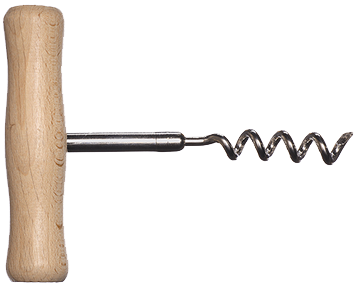
\includegraphics[]{corksckrew}};
    \draw [thick, red, decoration={
    									    markings,
    									    mark=at position 0.5 with {\arrow{latex}}}, postaction={decorate}](1.5,1.25) [ partial ellipse =5:355:0.25 and 1];
	 \draw[blue, -latex, thick] (3, 1.25) -- (4, 1.25) node[below] {$\vec{n}$} node[right, black] {рух гвинта};
	 \node[blue] at (2,2) {$N$};
	 \node[red] at (1,2) {$S$};
\end{tikzpicture}
\caption{Полюса витка}
\label{pic:gimlet}
\end{wrapfigure}
%---------------------------------------------------------

Магнітне поле впливає на магнітний диполь. Зокрема, на виток зі струмом, що вміщений в однорідне магнітне поле діє обертовий момент:
\begin{equation}\label{eq:Torque}
	\tcbhighmath[drop fuzzy shadow]{
	\vec{T} = \vec{p}_m\times \vec{B}.
	}
\end{equation}
Вираз~\eqref{eq:Torque} є фундаментальним фактом, тобто достовірність має бути перевірена на досліді.

Зокрема, вираз~\eqref{eq:Torque} дає можливість ввести кількісну характеристику  магнітного поля~--- \emph{вектора індукції}.

Для цього необхідно взяти виток з одиничним магнітним моментом, який ми визначили за формулою~\eqref{eq:circuit}. Для  того, щоб магнітний момент витка був одиничним, необхідно, щоб по ньому йшов струм в $I = 1$~Ампер, а площа такого витка дорівнювала $S = 1$~м$^2$. Розташуємо тепер виток так, щоб його магнітний момент був перпендикулярним до магнітного поля і виміряємо момент сили, тоді це значення і буде те число, яким ми кількісно охарактеризуємо магнітне поле\footnote{Характеристику магнітного поля --- індукцію --- не можна ввести аналогічно до того способу, яким вводиться характеристика електричного поля --- напруженість, тобто через силу, що діє на одиничний заряд, оскільки в природі не існує магнітного заряду (\href{https://en.wikipedia.org/wiki/Magnetic_monopole}{монополя}) }:
\begin{equation}\label{B}
	B = \frac{T}{p_m}.
\end{equation}
Ця величина назвається індукцією магнітного поля. В системі одиниць SI, ця величина вимірюється в Теслах, скорочено -- Tл:
\begin{equation}
	1 \text{Тл} = \frac{\text{1 Н}\cdot\text{м}}{\text{А}\cdot\text{м}^2}.
\end{equation}

\subsection{Котушки Гельмгольца}

Котушки Гельмгольца (кільця Гельмгольца) --- пристрій, що складається з двох однакових тонких соленоїдів, розташованих на одній осі на відстані один від одного, що дорівнює їх радіусам (рис.~\ref{pic:Helmholtz_coils}) і які з'єднані послідовно таким чином, щоб струм у них циркулював в однаковому напрямку. Котушка названа на честь \href{https://en.wikipedia.org/wiki/Hermann_von_Helmholtz}{Германа фон Гельмгольца}. Розташування двох соленоїдів на віддалі радіуса один від одного забезпечує таку однорідність поля вздовж осі, при якій відмінною від нуля є тільки четверта похідна від поля. Використовуються для отримання постійного, змінного або імпульсного магнітного поля з зоною однорідності, яке зазвичай використовується в експериментах, а також для калібрування датчиків магнітної індукції, намагнічування і розмагнічування постійних магнітів, розмагнічування сталевих заготівок, деталей і інструментів. Область поля з неоднорідністю менше $1$~\% є еліпсоїдом обертання близьким до сфери радіусом $0.3R$, що майже в $4$ рази більше ніж для одного кільця. Еліпсоїд трохи стислий уздовж осі (рис.~\ref{pic:Helmholtz_coils_field}).

%=========================================================
\begin{figure}[h!]\centering
%---------------------------------------------------------
\begin{minipage}[t]{0.45\linewidth}\centering
	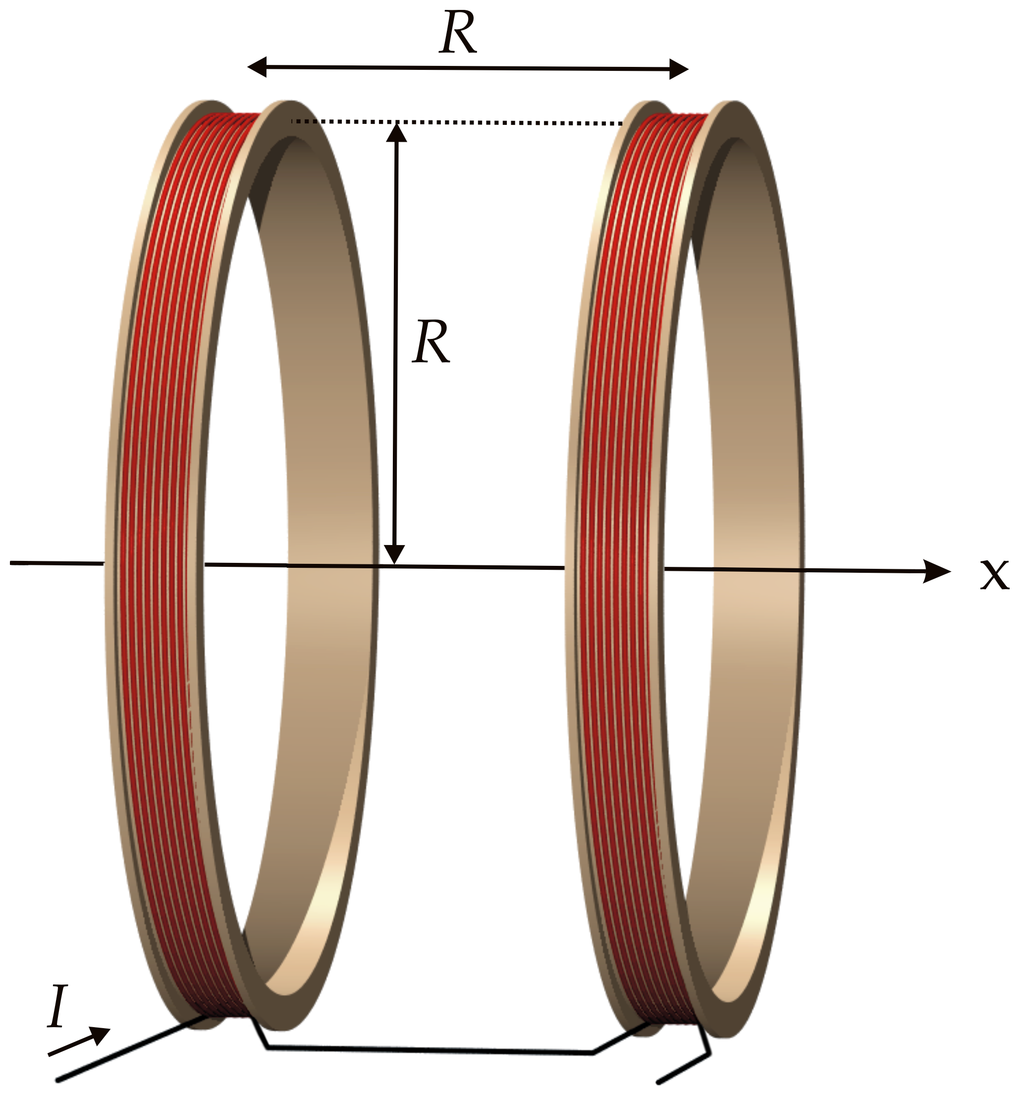
\includegraphics[width=0.8\linewidth]{Helmholtz_coils}
	\caption{Схема котушок Гельмгольца (взято з \href{https://en.wikipedia.org/wiki/Helmholtz_coil}{wikipedia})}
	\label{pic:Helmholtz_coils}
\end{minipage}
 \qquad%---------------------------------------------------------
\begin{minipage}[t]{0.45\linewidth}\centering
	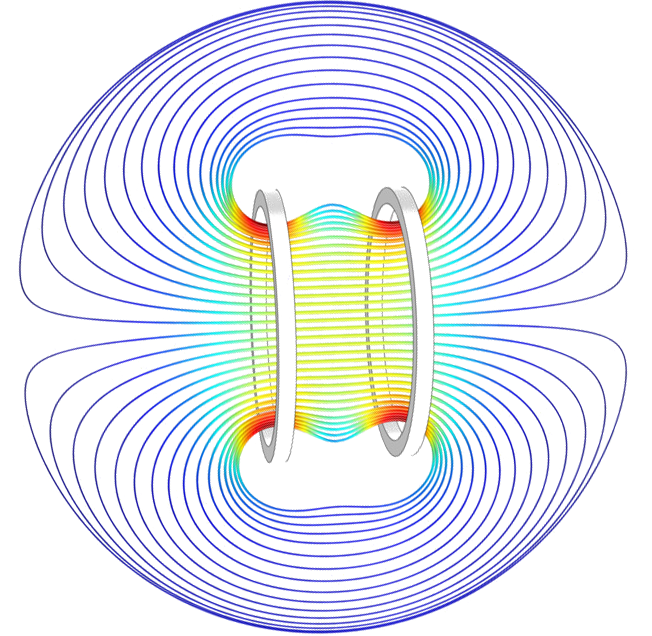
\includegraphics[width=0.8\linewidth]{Helmholtz_coils_field}
	\caption{Вигляд поля котушок Гельмгольца (взято з \href{https://www.freepng.ru/png-d02278/}{https://www.freepng.ru/png-d02278/})}
	\label{pic:Helmholtz_coils_field}
\end{minipage}
%---------------------------------------------------------
\end{figure}
%=========================================================

Магнітне поле в центрі між котушками можна розрахувати за допомогою закону Біо-Савара-Лапласа, який дає формулу:
\begin{equation}\label{eq:Helmholtz_coils_field}
\tcbhighmath[drop fuzzy shadow]{
B = \left( \frac45\right)^{\frac32} \frac{\mu_0 nI}{R}. 
}
\end{equation}
Константою котушок називається величина $C = \frac{B}{I}$, яка, як випливає з~\eqref{eq:Helmholtz_coils_field} визначається формулою:
\begin{equation}\label{eq:Helmholtz_coils_constant}
\tcbhighmath[drop fuzzy shadow]{
	C = \left( \frac45\right)^{\frac32} \frac{\mu_0 n}{R}, 
}
\end{equation}
де $n$~--- кількість витків в одному кільці, $R$~--- радіус кільця.

%
\pgfset{fpu}% ----- Увімкнення двигуна точних розрахунків
\pgfmathsetmacro{\muz}{4*pi*1e-7}
\pgfmathsetmacro{\R}{0.2}
\pgfmathsetmacro{\n}{154}
\pgfmathsetmacro{\CG}{(4/5)^(3/2)*\muz*\n/\R}
%
\begin{wraptable}{O}{0.65\linewidth}\small
	\centering
	\caption{Параметри котушок}
	\begin{tabular}{ll}
		\toprule
		Величина                         & Значення                              \\ \midrule
		Кількість витків в одному кільці & $n = \pgfmathprintnumber[]{\n}$       \\
		Радіус кільця                    & $R = \pgfmathprintnumber[]{\R}$ м     \\ \midrule
		Константа котушок                & $C = \pgfmathprintnumber[]{\CG}$ Тл/А \\ \bottomrule
	\end{tabular}
	\label{tab:Helmgoltz_coils}
\end{wraptable}
В даній лабораторній роботі використовуються котушки Гельмгольца, параметри яких подані в  табл.~\ref{tab:Helmgoltz_coils}.


Розраховане значення константи котушок за формулою~\eqref{eq:Helmholtz_coils_constant} з використанням даних таблиці~\ref{tab:Helmgoltz_coils} дає значення:

\begin{equation*}
	C = \pgfmathparse{\CG}\pgfmathprintnumber[sci, precision=2]{\pgfmathresult}~\text{Тл/А}.
\end{equation*}
\pgfset{fpu=false}% ----- Вимкнення двигуна точних розрахунків

\section{Хід роботи}

\begin{enumerate}
	\item Збираємо лабораторну установку (рис.~\ref{pic:Experimental_installation}). Одне джерело струму (рис.~\ref{pic:Power_supply}) через амперметр приєднується до котушок Гельмгольца (рис.~\ref{pic:scheme_for_Helmholtz}), інше --- до контуру (рис.~\ref{pic:scheme_for_coil}). Треба простежити, щоб провідники, які підводять струм до контуру не спричиняли додатковий обертальний момент. Крутильні терези мають бути встановлені таким чином, щоб контур знаходився точно в центрі між котушками.

%=========================================================
\begin{figure}[h!]\centering
%---------------------------------------------------------
\begin{minipage}[t]{0.47\linewidth}
\begin{tornpage}\centering
		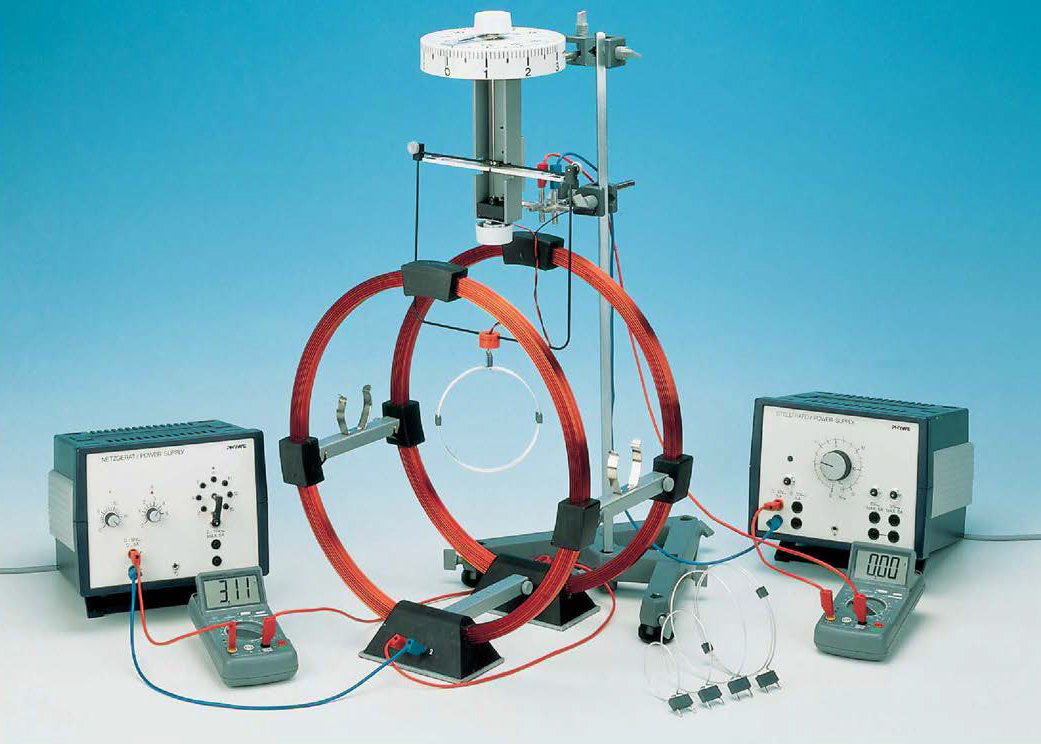
\includegraphics[width=1\linewidth]{Experimental_installation}
		\caption{Експериментальна установка}
		\label{pic:Experimental_installation}
\end{tornpage}
\end{minipage}
\quad%---------------------------------------------------------
\begin{minipage}[t]{0.47\linewidth}
\begin{tornpage}\centering
		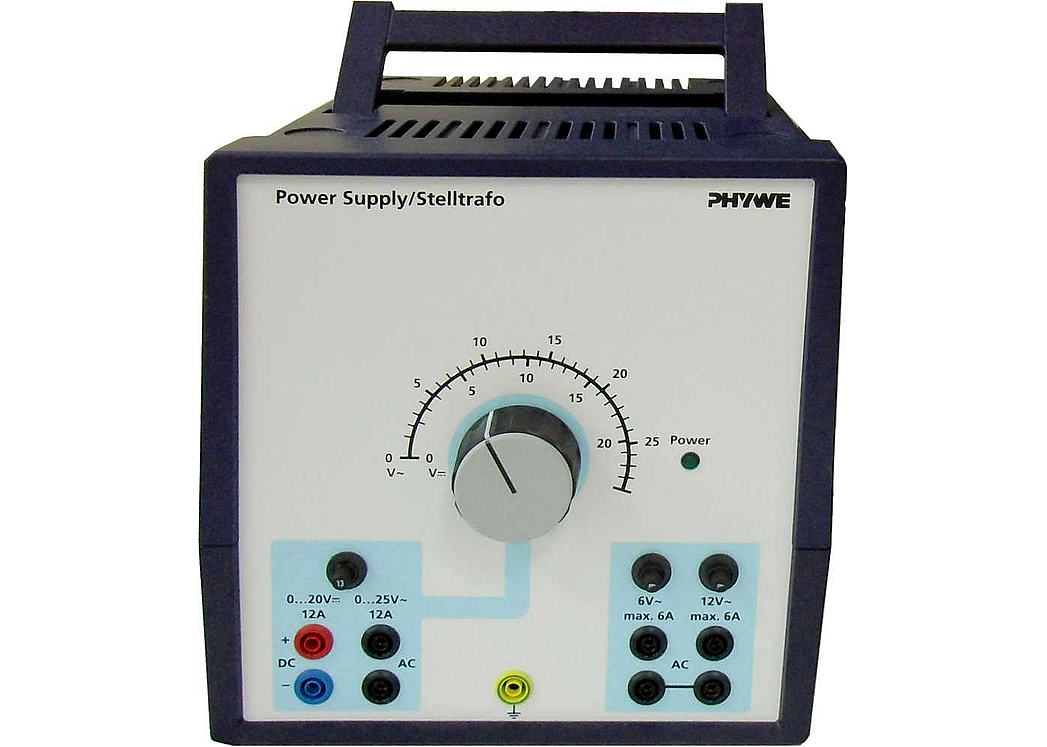
\includegraphics[width=1\linewidth]{Power_supply}
		\caption{Джерело живлення}
		\label{pic:Power_supply}
\end{tornpage}
\end{minipage}
%---------------------------------------------------------
\end{figure}

%=========================================================
\begin{figure}[h!]\centering
%---------------------------------------------------------
\begin{minipage}[t]{0.45\linewidth}\centering
	\begin{tikzpicture}[scale=1.5]
		\draw  (0,0) node[contact] {} -- ++(0,1) to[ampermeter] ++(4,0) -- ++(0,-1) -- ++(-0.5,0) node[above right] {$2$};
		\draw  (0,-1) node[contact] {} -- ++(0,-1) -- ++(2.25,0) -- ++(0,1)  -- ++(0.5,0) node[below left] {$2$};
		\fill[red!50, draw=red] (3.3,0.25) rectangle +(0.2,-1.5);
		\fill[red!50, draw=red] (2.75,0.25) rectangle +(0.2,-1.5);
		\draw (2.75,0) node[above left] {$1$} -- ++(-0.5,0)  -- ++(0,0.5) -- ++(0.85,0) -- ++(0,-2) -- ++(0.9,0)  -- ++(0,0.5)  -- ++(-0.5,0) node[below right] {$1$};
		\node at (0,-0.5) {$I \le 3$~А};
	\end{tikzpicture}
\caption{Схема з'єднання котушок}
\label{pic:scheme_for_Helmholtz}
\end{minipage}
%---------------------------------------------------------
\begin{minipage}[t]{0.45\linewidth}\centering
	\begin{tikzpicture}[scale=1.5]
		\draw  (0,0) node[contact] {} -- ++(0,0.9) to[ampermeter] ++(2,0) -- ++(0,-1.25) -- ++(0.5,0) coordinate (A) ;
		\draw  (0,-1) node[contact] {} -- ++(0,-0.9) to [resistor={adjustable}] ++(2,0) -- ++(0,1.25) -- ++(0.5,0) coordinate (B) ;
		\draw[ultra thick, red!30] ([shift={(0.47,-0.22)}]A) circle (0.5);
		\draw[ultra thick, red!30] ([shift={(0.47,-0.27)}]A) circle (0.5);
		\draw[ultra thick, red!50] (A) node[contact] {} ++(180:0) arc (160:-165:0.5) node[contact] {};
		\node at (0,-0.5) {$I \le 2$~A};
	\end{tikzpicture}
\caption{Схема з'єднання контура}
\label{pic:scheme_for_coil}
\end{minipage}
%---------------------------------------------------------
\end{figure}
%=========================================================


	\item Зніміть залежність обертального моменту від сили струму в контурі.
	\item \ldots
\end{enumerate}

\section{Результи вимірювань та обробка експериментальних даних}

\subsection{Визначення залежності обертального моменту від струму в контурі $T(I)$}

%========================================== Вихідні дані експерименту ====================================================%
%
Константи експерименту наведені в табл.~\ref{tab:expcont}.

\pgfmathsetmacro{\N}{3}
\pgfmathsetmacro{\D}{0.12}
\pgfmathsetmacro{\angle}{90}
\pgfmathsetmacro{\IG}{2.85}

%\begin{table}[h!]
%	\centering
%	\caption{Константи експерименту}
%	\begin{tabular}{ll}
%		\toprule
%		Величина                                 & Значення                        \\ \midrule
%		Число витків контура, $N$            & $\pgfmathprintnumber[]{\N}$     \\
%		Діаметр контура, $D$, м                  & $\pgfmathprintnumber[]{\D}$     \\
%		Струм в котушках, $I'$, А    & $\pgfmathprintnumber[]{\IG}$    \\ 
%		Орієнтація контура, $\alpha$, ${}^\circ$ & $\pgfmathprintnumber[]{\angle}$ \\ \bottomrule
%	\end{tabular}
%	\label{tab:expcont}
%\end{table}
%
%==========================================================================================================================%

Було виміряно момент сили, що діє на контур зі струмом в магнітному полі. Оскільки динамометр прилада градуйований в мН, то для отримання значення моменту, вказані значення сили необхідно домножити на плече, що дорівнює $12$~см.

%Результати вимірювань наведені в табл.~\ref{tab:expresults}.
%========================================== Завантаження данних з таблиці ===================================================%
%----- Присвоєння данних змінній \TorqueVsCurrentTable
\pgfplotstableread{
Current Force    FError
0     0          0
0.5   0.40e-03   0.05e-3
1     0.70e-03   0.05e-3
1.5   1.00e-03   0.05e-3
1.9   1.30e-03   0.05e-3
1.7   1.20e-03   0.05e-3
1.2   0.75e-03   0.10e-3
0.8   0.60e-03   0.05e-3
}\TorqueVsCurrentTable
%========================================== Додавання нової колонки в таблицю =============================================%
%----- Додається нова колонка Torque (обертовий момент), значення в якій є результатом множення колонки Force (Сила) на 0.12
\pgfplotstablecreatecol[
	create col/expr={\thisrow{Force}*0.12},
]{Torque}\TorqueVsCurrentTable

%========================================== Додавання нової колонки в таблицю =============================================%
%----- Додається нова колонка TError (похибка для обертового моменту), значення в якій є результатом множення колонки FError (похибки для сили) на 0.12
\pgfplotstablecreatecol[
	create col/expr={\thisrow{FError}*0.12},
]{TError}\TorqueVsCurrentTable

%========================================== Побудова таблиці для відображення =============================================%
%\begin{table}[h!]
%	\centering
%	\caption{Результати вимірювань}
%	\label{tab:expresults}
%	\pgfplotstabletypeset[
%		col sep=space,
%		%1000 sep={,},
%		every head row/.style={
%				before row={\toprule},
%				after row={\midrule}
%			},
%		every last row/.style={after row=\bottomrule},
%		empty cells with={-},
%		columns/Current/.style={fixed zerofill, dec sep align, sci precision=2, column name={$I$, А}, },
%		columns={Force,Torque, Current},
%		columns/Force/.style={fixed zerofill, sci precision=1, column name={$F$, $\cdot 10^{-3}$ Н}, multiply by=1000},
%		columns/Torque/.style={fixed zerofill, sci precision=1, column name={$T$, $\cdot 10^{-4}$ Н$\cdot$м}, multiply by=1e4},
%	]\TorqueVsCurrentTable
%\end{table}
%
%==========================================================================================================================%

За даними результатами побудуємо графік~\ref{plt:expresults}.

\begin{tornpage}
\begin{center}%[h!]
	%\centering
	\begin{tikzpicture}
		\begin{axis}[legend style={font=\scriptsize},
				xlabel={$I$, А},
				ylabel=\empty,
%				every axis y label/.style={
%				    at={(yticklabel cs:1)},
%				    anchor=south,
%				},
				every y tick scale label/.style={at={(0.05,1)},anchor=south},
				ytick scale label code/.code={$T$, $\cdot 10^{#1}$ Н$\cdot$м},
				%	xmin = 3,
				%	xmax = 8,
				legend pos = north west,
				minor tick num = 2,
				width=1\linewidth,
				height=0.6\linewidth,
				% === Налаштування сітки ===
				grid = both,
				grid style={line width=.1pt, draw=gray!10},
				major grid style={line width=.2pt,draw=gray!50},
				minor tick num = 5,
				minor grid style = {line width=.1pt,draw=gray!10},
			]

%-------------------------------------------- Побудова графіку за даними з файлу -----------------------------------------%
%
			\addplot[
				blue,
				only marks,
				error bars/.cd,
				y dir = both,  y explicit,
			]
			table[
					x=Current,
					y expr={\thisrow{Torque}},
					y error = TError,
				]\TorqueVsCurrentTable;

%------------------------------------ Додавання легенди до вищепобудованого графіку --------------------------------------%
			\addlegendentry{Експериментальні дані}

%---------------------------------- Побудова лінійної апроксимації до даних файлу ----------------------------------------%	
			\addplot[red,
			]
			table[x=Current, y={create col/linear regression={y = Torque}}]\TorqueVsCurrentTable;
			\xdef\slope{\pgfplotstableregressiona}
			\xdef\ycepte{\pgfplotstableregressionb}

%------------------------------------ Додавання легенди до вищепобудованого графіку --------------------------------------%
			\addlegendentry{
				$T = \pgfmathprintnumber{\slope} \cdot I \pgfmathprintnumber[print sign]{\ycepte}$
				Апроксимація
			}
%------------------------------------ Додавання таблиці з даними на графік -----------------------------------------------%
			\node [above left,
				text width=6.7cm,
				align=center] at ([xshift=-0.2cm,yshift=0.1cm]current axis.south east) {%
				\begin{tornpage}
				\vspace*{-0.7\baselineskip}% a bit of a ugly hack, the \captionof seems to make an empty line at the start of the node
				\scriptsize%
				\centering%
				\captionsetup[table]{font=scriptsize, labelfont=scriptsize}
				\captionof{table}{Константи експерименту}
				\begin{tabular}{ll}
					\toprule
					Величина             & Значення                                       \\ \midrule
					Число витків контура & $N = \pgfmathprintnumber[]{\N}$                \\
					Діаметр контура      & $D = \pgfmathprintnumber[]{\D}$ м              \\
					Струм в котушках     & $I'= \pgfmathprintnumber[]{\IG}$ А             \\
					Орієнтація контура   & $\alpha = \pgfmathprintnumber[]{\angle}^\circ$ \\ \bottomrule
				\end{tabular}
				\label{tab:expcont}
				\end{tornpage}
				};		
	\end{axis}
	\end{tikzpicture}
	\captionof{figure}{Графік залежності обертального моменту від струму у витку $T(I)$.}
	\label{plt:expresults}
\end{center}
\end{tornpage}
%
%=========================================================================================================================%

Обчислюємо константу котушок Гельмгольца з даних апроксимації%
\footnote{%
Тут прийдеться зробити апроксимацію експериментальних даних прямою $y = kx + b$. З теорії ясно, апроксимована залежність має проходити через початок координат, тобто $b = 0$. Проте, при обробці таких даних не можна використовувати залежність виду $y = kx$, оскільки це еквівалентно додаванню неіснуючих експериментальних точок до реально виміряного набору даних. Більш того, апроксимація експериментальних даних залежністю виду $y = kx + b$ дозволяє визначити систематичну похибку, яка присутня в вимірах. Якщо величина $b$ не дорівнює нулю, і <<нуль>> не попадає всередину діапазону похибки $\pm\Delta b$, то слід зробити висновок, що або прийнята модель (тобто що $y = kx$) невірна, або точність проведених експериментів (наприклад, неврахована систематична похибка ) більше статистичної та неможливо з необхідною точністю визначити величину $k$. Для більш точного визначення величини $k$ необхідно, як правило, розширити діапазон зміни $x$ в експерименті, якщо ж це не покращує ситуацію, то необхідно перевірити, чи немає інших джерел систематичної помилки.}.

\pgfset{fpu}% ----- Увімкнення двигуна точних розрахунків

Для даного експерименту, константу котушок можна визначити, знаючи коефіцієнт апроксимації $k \approx \pgfmathprintnumber[sci, precision=1]{\slope}\,\frac{\text{Н}\cdot\text{м}}{\text{А}}$ згідно формули:
\begin{equation}\label{capour}
	C = \frac{4k}{IN\pi D^2}
\end{equation}

Обчислення дають значення:
%----------------------------------------------- Математичні обчислення --------------------------------------------------%
\pgfmathsetmacro{\HelmholtzConstant}{4*\slope/(\IG*\N*\D*\D*pi*sin(\angle))}% ----- Обчислення значення
\pgfmathfloatparsenumber{\HelmholtzConstant}% ---- Розпарсити число на мантісу m і експонетну e у вигляді: m*10^e
\pgfmathfloattomacro{\pgfmathresult}{\FlagHC}{\MantissaHC}{\ExponentHC}% --- Запис мантиси і експоненти у відповідні змінні
%-------------------------------------------------------------------------------------------------------------------------%
\begin{equation*}
	C \approx  
	(\pgfmathprintnumber[fixed, precision=1]{\MantissaHC} \pm 1.2) \cdot 10^{\ExponentHC} \text{~Тл/А}
\end{equation*}


Відносна похибка:%
\pgfmathparse{(1.22e-4/\HelmholtzConstant)*100}
\begin{equation*}
	\epsilon \approx \pgfmathprintnumber[fixed, precision=0]{\pgfmathresult}~\text{\%}.
\end{equation*}

\pgfset{fpu=false}% ----- Вимкнення двигуна точних розрахунків

\section{Обговорення результатів}



За результатами експериментів було перевірено формулу~\eqref{eq:Torque}. Із результатів експериментів випливає, що формула вірна в межах вказаної точності. За результатами дослідів було знайдено константу котушок Гельмгольца. Порівняння знайденого значення із теоретично обрахованим за законом Біо-Савара-Лапласа показує дещо завищене її значення, навіть якщо рахувати по нижній межі експериментальної похибки. Оскільки похибка теоретичне теоретично обрахованого значення залежить лише від точності вимірювань геометричних параметрів, то можна визначити, що ця оцінка не перевищує значення $0.1$~\%. Причини високої  експериментальної високої похибки та завищеного значення константи котушок, як показують додаткові дослідження можуть полягати в \ldots


\section*{Висновки}

\end{document}
